\chapter{Thực nghiệm và phân tích kết quả}
\section{Điều kiện thực nghiệm}
Các thực nghiệm chạy trên CPU với Python 3.11.9, PyTorch 2.15.0+cpu, scikit-learn 1.9.1, pandas 2.3.3 và Streamlit 1.66.1. Phiên bản trực tiếp được ghi trong requirements, còn môi trường kiểm tra đầy đủ nằm ở \texttt{artifacts/environment.txt}. Môi trường cài mới trên máy khác chưa được kiểm chứng; việc bàn giao xác nhận source và artifact chạy trong môi trường nêu trên.

Dữ liệu supervised dùng một split/seed cố định. RL chạy năm seed train và các seed eval tách biệt. Đánh giá phần mềm và truy xuất sử dụng kịch bản do tác giả xây. Mỗi loại bằng chứng trả lời một câu hỏi khác nhau: test supervised đo phân loại nội bộ, simulator đo utility giả định, bộ tình huống đo tuân thủ hợp đồng. Không gộp các điểm này thành một tỷ lệ chính xác chung của hệ thống y tế.

\section{Kết quả validation và lựa chọn mặc định}
\begin{table}[H]\centering\small
\caption{Chỉ số trên validation; ngưỡng được chọn bằng F1 validation.}
\begin{tabular}{@{}lrrrrrr@{}}\toprule
Model & AUC & AP & F1 & Precision & Recall & Brier \\\midrule
dummy & 0.5000 & 0.1314 & 0.2322 & 0.1314 & 1.0000 & 0.1142 \\
logistic & 0.8127 & 0.3482 & 0.4350 & 0.3397 & 0.6047 & 0.0986 \\
random\_forest & 0.8104 & 0.3713 & 0.4387 & 0.3383 & 0.6237 & 0.0967 \\
mlp & 0.8170 & 0.3706 & 0.4414 & 0.3285 & 0.6723 & 0.0960 \\
\bottomrule\end{tabular}
\end{table}
Random Forest có Average Precision validation khoảng 0,3713, nhỉnh hơn MLP khoảng 0,3706. Theo quy tắc đã đặt, Random Forest được chọn làm model mặc định. MLP có ROC AUC validation cao hơn, nhưng tiêu chí chọn đã khóa là AP nên không đổi sang AUC sau khi thấy bảng kết quả.

Chênh lệch AP giữa hai model rất nhỏ và chưa có phân tích độ bất định để kết luận model nào tốt hơn ổn định. Lựa chọn mặc định chỉ là kết quả áp dụng quy tắc trong lần chia tập này. Giao diện vẫn cho chọn MLP để trình diễn nhánh học sâu và so sánh với các baseline.

\section{Kết quả trên test đã khóa}
\begin{table}[H]\centering\small
\caption{Chỉ số trên test; ngưỡng được chọn bằng F1 validation.}
\begin{tabular}{@{}lrrrrrr@{}}\toprule
Model & AUC & AP & F1 & Precision & Recall & Brier \\\midrule
dummy & 0.5000 & 0.1373 & 0.2415 & 0.1373 & 1.0000 & 0.1185 \\
logistic & 0.8118 & 0.3820 & 0.4367 & 0.3499 & 0.5806 & 0.1003 \\
random\_forest & 0.8096 & 0.3906 & 0.4534 & 0.3564 & 0.6230 & 0.0993 \\
mlp & 0.8168 & 0.3916 & 0.4431 & 0.3358 & 0.6512 & 0.0987 \\
\bottomrule\end{tabular}
\end{table}
\begin{table}[H]\centering\small
\caption{Ngưỡng đã khóa và số lượng dự đoán trên test.}
\begin{tabular}{@{}lrrrrrr@{}}\toprule
Model & Ngưỡng & TN & FP & FN & TP & Specificity \\\midrule
dummy & 0.050 & 0 & 3116 & 0 & 496 & 0.0000 \\
logistic & 0.215 & 2581 & 535 & 208 & 288 & 0.8283 \\
random\_forest & 0.230 & 2558 & 558 & 187 & 309 & 0.8209 \\
mlp & 0.205 & 2477 & 639 & 173 & 323 & 0.7949 \\
\bottomrule\end{tabular}
\end{table}

\noindent\textbf{Quan sát.} MLP đạt ROC AUC khoảng 0,8168 và AP khoảng 0,3916; Random Forest đạt AUC khoảng 0,8096 và AP khoảng 0,3906. Logistic Regression đạt AUC khoảng 0,8118. Các model học được đều có AP cao hơn Dummy khoảng 0,1373, là tỷ lệ lớp dương trong test.

\noindent\textbf{Diễn giải.} MLP nhỉnh hơn về AUC/AP trên test nhưng không làm thay đổi quyết định mặc định đã khóa từ validation. Các chênh lệch này là mô tả trên cùng split, chưa đủ để khẳng định ưu thế tổng quát. Mô hình bảng đơn giản hơn vẫn là đối chứng cần thiết cho một mạng hai lớp ẩn.

\noindent\textbf{Đánh đổi tại ngưỡng.} MLP phát hiện 323/496 mẫu lớp 1, còn bỏ sót 173 mẫu và tạo 639 dương tính giả. Random Forest phát hiện 309 mẫu, bỏ sót 187 và tạo 558 dương tính giả. Khi tăng recall, precision có thể giảm; việc chọn F1 validation không đồng nghĩa chọn ngưỡng phù hợp cho quyết định lâm sàng.

\begin{figure}[H]\centering
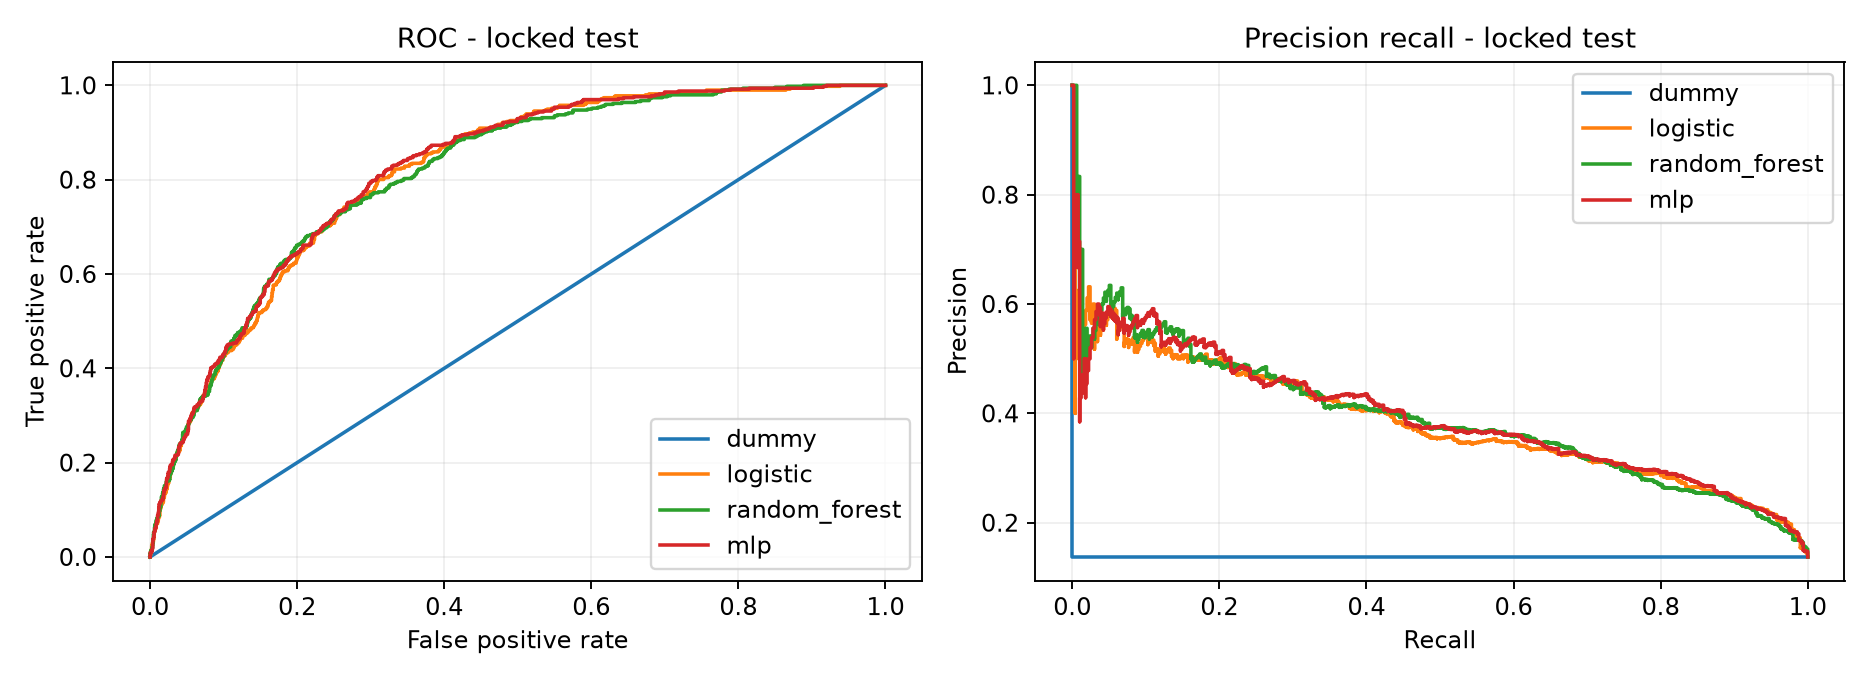
\includegraphics[width=\textwidth]{images/classification.png}
\caption{ROC và Precision--Recall trên test. Mọi quyết định về model/ngưỡng được thực hiện bằng validation trước đó.}
\end{figure}

Dummy được chọn ngưỡng nhỏ hơn điểm tiên nghiệm nên dự đoán tất cả là lớp 1, dẫn tới recall 1 và specificity 0. Điều này minh họa vì sao một chỉ số riêng lẻ có thể gây hiểu nhầm. Cần đọc đồng thời precision, recall và số lượng FP/FN.

\section{Quá trình học của MLP}
\begin{figure}[H]\centering
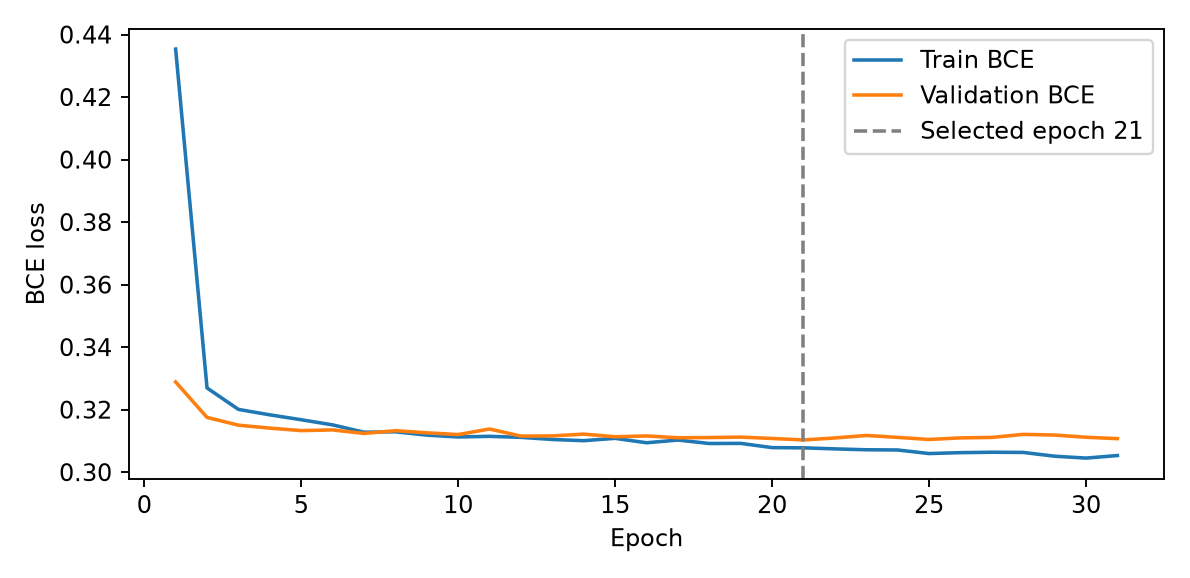
\includegraphics[width=0.92\textwidth]{images/training.png}
\caption{Loss train và validation, đường dọc thể hiện epoch được chọn để lưu checkpoint.}
\end{figure}

Checkpoint MLP được chọn tại epoch 21 theo BCE validation. Train tiếp tục cho tới khi đủ số epoch không cải thiện rồi nạp lại checkpoint tốt nhất. Train loss và validation loss không nhất thiết cùng giảm ở các epoch cuối; đó là lý do giữ checkpoint dựa trên tập không tham gia cập nhật gradient.

Brier test của MLP khoảng 0,0987, thấp hơn Dummy khoảng 0,1185. Đây là dấu hiệu mô hình cung cấp score hữu ích hơn tiên nghiệm trong điều kiện test nội bộ. Chưa có đường calibration theo nhóm, khoảng tin cậy hoặc đánh giá dịch chuyển phân bố nên không thể chuyển score đó thành nguy cơ cá nhân ở Việt Nam.

\section{Truy xuất tri thức và vai trò đồ thị}
\begin{table}[H]\centering\small
\caption{Đánh giá truy xuất trên 24 câu hỏi của bộ thực nghiệm.}
\begin{tabular}{@{}lrrr@{}}\toprule
Cấu hình & Hit@1 & Hit@3 & MRR \\\midrule
TF-IDF & 1.0000 & 1.0000 & 1.0000 \\
TF-IDF + graph & 1.0000 & 1.0000 & 1.0000 \\
\bottomrule\end{tabular}
\end{table}

Cả hai cấu hình đều tìm đúng ID đầu tiên ở toàn bộ 24 câu trong phiên bản cuối. Vì vậy, bộ câu hiện tại không cho thấy lợi ích đo được của bonus đồ thị về Hit@1, Hit@3 hoặc MRR. Đồ thị vẫn có chức năng biểu diễn liên kết và mở rộng concept trong implementation, nhưng chưa có bằng chứng nó làm tăng chất lượng trên tập kiểm tra này.

Điểm tuyệt đối cần được đọc cùng giới hạn thiết kế: chỉ 12 ghi chú, câu hỏi do chính tác giả viết và dùng lại để kiểm tra trong phát triển. Không có bộ paraphrase độc lập hoặc đánh giá từ người dùng. Một bước tiếp theo có giá trị là thu thập câu hỏi ngoài từ vựng KB, nhiều chủ đề và trường hợp cần từ chối, rồi khóa bộ test riêng.

\section{Kết quả Q-learning và đối chứng}
\begin{table}[H]\centering\small
\caption{Reward mỗi ngày trong simulator; std giữa năm giá trị trung bình theo seed train.}
\begin{tabular}{@{}lrr@{}}\toprule
Policy & Reward trung bình & Độ lệch chuẩn \\\midrule
fixed & 0.2868 & 0.0000 \\
never & 0.0876 & 0.0000 \\
q\_learning & 0.2703 & 0.0153 \\
rule & 0.2006 & 0.0000 \\
\bottomrule\end{tabular}
\end{table}
\begin{figure}[H]\centering
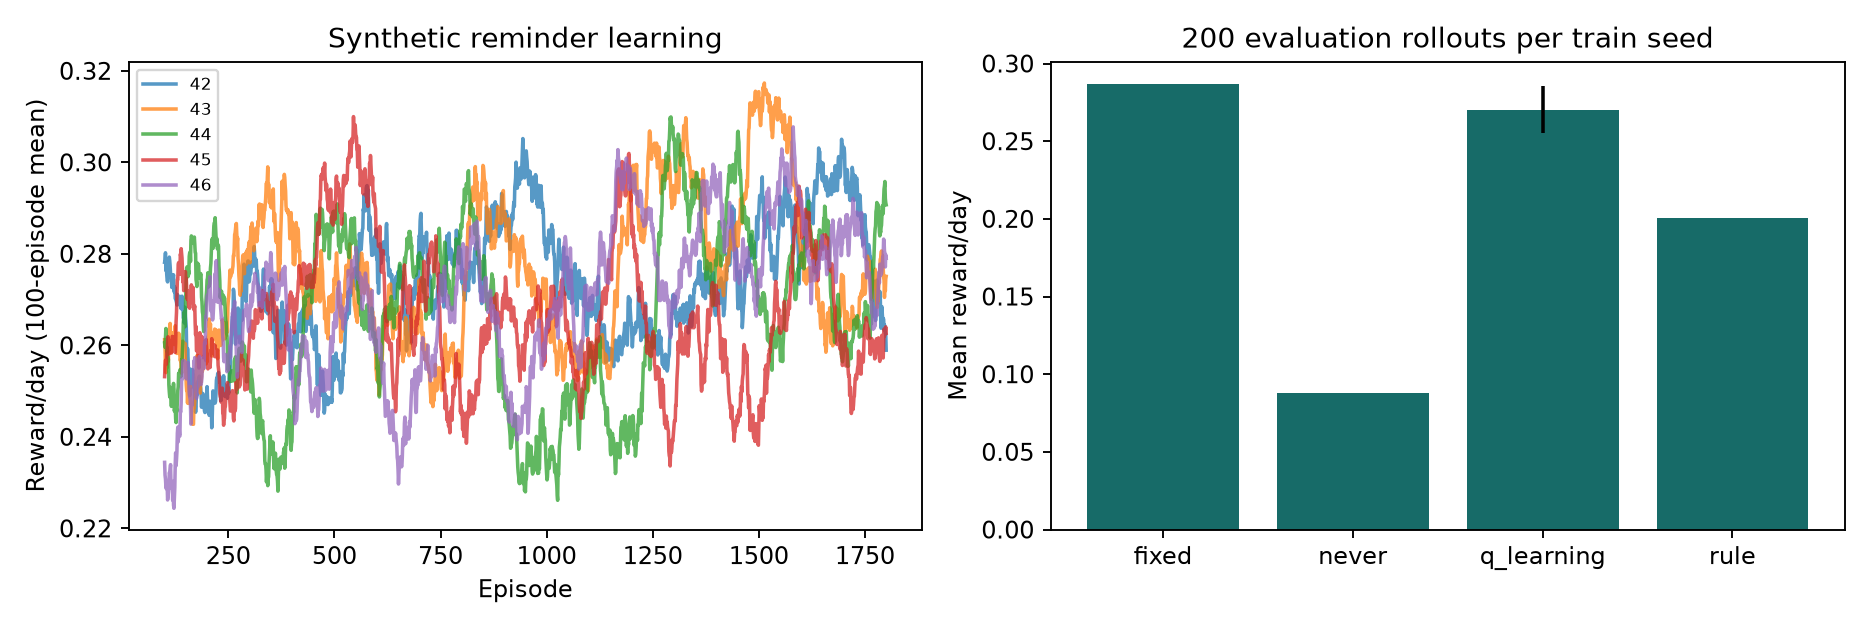
\includegraphics[width=\textwidth]{images/rl.png}
\caption{Đường học năm seed và reward đánh giá trong môi trường nhắc việc giả lập.}
\end{figure}

\noindent\textbf{Quan sát.} Q-learning có reward trung bình khoảng 0,2703 mỗi ngày, cao hơn never khoảng 0,0876 và rule khoảng 0,2006, nhưng thấp hơn fixed khoảng 0,2868. Độ lệch chuẩn giữa năm seed train của Q-learning khoảng 0,0153.

\noindent\textbf{Diễn giải.} Trong simulator này, lợi ích ghi nhận do hành động nhắc thường bù được chi phí nên policy luôn nhắc là đối chứng mạnh. Q-learning hữu hạn với learning rate cố định và năm seed chưa vượt đối chứng đó. Kết quả không được sửa bằng cách đổi reward sau khi xem điểm; báo cáo giữ nguyên cả trường hợp RL không tốt nhất.

\noindent\textbf{Giới hạn của phép đo.} Fixed/never/rule có std giữa seed train bằng 0 vì cùng policy được đánh giá lại với cùng 200 seed eval, không phải vì mọi rollout có reward giống nhau. Các dòng lặp của đối chứng không tạo thêm mẫu độc lập. Q-table seed 42 được nạp trong demo theo quy ước trước, không chọn theo reward eval.

\section{Kiểm tra tích hợp và lỗi được inject}
\begin{table}[H]\centering\small
\caption{Các kịch bản chức năng được chạy ở phiên bản bàn giao.}
\begin{tabular}{@{}llcr@{}}\toprule
Kịch bản & Trạng thái mong đợi & Đạt & Thông điệp \\\midrule
risk\_complete & completed & Có & 8 \\
risk\_mlp & completed & Có & 8 \\
risk\_missing & needs\_input & Có & 8 \\
risk\_invalid & needs\_input & Có & 8 \\
risk\_nan & needs\_input & Có & 8 \\
knowledge\_a1c & completed & Có & 8 \\
knowledge\_food & completed & Có & 8 \\
knowledge\_activity & completed & Có & 8 \\
knowledge\_unknown & insufficient\_evidence & Có & 8 \\
knowledge\_blank & insufficient\_evidence & Có & 8 \\
urgent\_text & urgent & Có & 2 \\
urgent\_seizure & urgent & Có & 2 \\
urgent\_glucose & urgent & Có & 2 \\
invalid\_unit\_value & needs\_input & Có & 2 \\
medication & out\_of\_scope & Có & 2 \\
reminder & completed & Có & 8 \\
invalid\_reminder & needs\_input & Có & 8 \\
consult & completed & Có & 12 \\
consult\_missing & needs\_input & Có & 12 \\
consult\_unknown & insufficient\_evidence & Có & 12 \\
\bottomrule\end{tabular}
\end{table}
Toàn bộ 20 kịch bản đạt trạng thái mong đợi ở phiên bản bàn giao. Kịch bản phủ luồng dự đoán, dữ liệu thiếu/sai mã, query có/không có bằng chứng, số đo bổ sung không hợp lệ, nhánh khẩn cấp, phạm vi thuốc và reminder. Đây là tỷ lệ đạt bộ yêu cầu phần mềm hữu hạn, không phải tỷ lệ tư vấn đúng trong mọi tình huống.

Sáu proposal lỗi được inject riêng gồm thuốc, tri thức không nguồn, ID giả, score vượt khoảng, score NaN và lỗi handler. Council bác cả sáu. Ở cấu hình bỏ Council, các proposal được đánh dấu unreviewed; không gọi đó là đã qua kiểm tra hoặc đã gây hại. Phép ablation xác nhận chức năng veto đối với lỗi được dựng sẵn, chưa chứng minh MAS tốt hơn một pipeline đơn tác tử dùng cùng luật và công cụ.

\section{Kiểm thử tự động và notebook}
Bộ pytest có 28 trường hợp và đều đạt. Các nhóm kiểm tra gồm checksum/fingerprint, mã khảo sát không hợp lệ, score nạp lại khớp prediction, ưu tiên urgent trước Risk, nguồn cảnh báo glucose, truy xuất không dấu và từ chối ngoài chủ đề, Council veto, cô lập exception trong bus, tính tái lập Q, miền trạng thái, ghi/đọc audit và thao tác UI bằng Streamlit AppTest.

Bốn notebook có lần lượt 7, 6, 5 và 8 code cell, tổng cộng 26 cell. Tất cả có execution count và không có error output. Log lưu tên file, số cell và thời gian thực thi. Việc kiểm tra trực tiếp bằng trình duyệt còn được dùng để quan sát màu chữ, bố cục và ảnh minh chứng, bổ sung cho kiểm thử cấu trúc bằng AppTest.

